\documentclass[a4paper,11pt]{book}
%\documentclass[a4paper,twoside,11pt,titlepage]{book}
\usepackage{listings}
\usepackage[utf8]{inputenc}
\usepackage[spanish]{babel}

% \usepackage[style=list, number=none]{glossary} %
%\usepackage{titlesec}
%\usepackage{pailatino}

\decimalpoint
\usepackage{dcolumn}
\usepackage{float}
\newcolumntype{.}{D{.}{\esperiod}{-1}}
\makeatletter
\addto\shorthandsspanish{\let\esperiod\es@period@code}
\makeatother


%\usepackage[chapter]{algorithm}
\RequirePackage{verbatim}
%\RequirePackage[Glenn]{fncychap}
\usepackage{fancyhdr}
\usepackage{graphicx}
\usepackage{afterpage}
\usepackage{longtable}

\usepackage[pdfborder={000}]{hyperref} %referencia

% ********************************************************************
% Re-usable information
% ********************************************************************
\newcommand{\myTitle}{Deep Learning para diagnóstico a partir de imágenes Biomédicas\xspace}
\newcommand{\myDegree}{Grado en Ingeniería Informática\xspace}
\newcommand{\myName}{Francisco Carrillo Pérez \xspace}
\newcommand{\myProf}{Luis Javier Herrera Maldonado\xspace}
\newcommand{\myOtherProf}{Alberto Guillén Perales (tutor2)\xspace}
%\newcommand{\mySupervisor}{Put name here\xspace}
\newcommand{\myFaculty}{Escuela Técnica Superior de Ingenierías Informática y de
Telecomunicación\xspace}
\newcommand{\myFacultyShort}{E.T.S. de Ingenierías Informática y de
Telecomunicación\xspace}
\newcommand{\myDepartment}{Departamento de Arquitectura de Computadores\xspace}
\newcommand{\myUni}{\protect{Universidad de Granada}\xspace}
\newcommand{\myLocation}{Granada\xspace}
\newcommand{\myTime}{\today\xspace}
\newcommand{\myVersion}{Version 0.1\xspace}


%\hypersetup{
%pdfauthor = {\myName franciscocp@correo.ugr.es},
%pdftitle = {\myTitle},
%pdfsubject = {},
%pdfkeywords = {palabra_clave1, palabra_clave2, palabra_clave3, ...},
%pdfcreator = {LaTeX con el paquete ....},
%pdfproducer = {pdflatex}
%}

%\hyphenation{}


%\usepackage{doxygen/doxygen}
\usepackage{pdfpages}
\usepackage{url}
\usepackage{colortbl,longtable}
\usepackage[stable]{footmisc}
%\usepackage{index}
%\makeindex
%\usepackage[style=long, cols=2,border=plain,toc=true,number=none]{glossary}
%\makeglossary

% Definición de comandos que me son tiles:
%\renewcommand{\indexname}{Índice alfabético}
%\renewcommand{\glossaryname}{Glosario}

\pagestyle{fancy}
\fancyhf{}
\fancyhead[LO]{\leftmark}
\fancyhead[RE]{\rightmark}
\fancyhead[LE]{\textbf{\thepage}}
\renewcommand{\chaptermark}[1]{\markboth{\textbf{#1}}{}}
\renewcommand{\sectionmark}[1]{\markright{\textbf{\thesection. #1}}}

\setlength{\headheight}{1.5\headheight}

\newcommand{\HRule}{\rule{\linewidth}{0.5mm}}
%Definimos los tipos teorema, ejemplo y definición podremos usar estos tipos
%simplemente poniendo \begin{teorema} \end{teorema} ...
\newtheorem{teorema}{Teorema}[chapter]
\newtheorem{ejemplo}{Ejemplo}[chapter]
\newtheorem{definicion}{Definición}[chapter]

\definecolor{gray97}{gray}{.97}
\definecolor{gray75}{gray}{.75}
\definecolor{gray45}{gray}{.45}
\definecolor{gray30}{gray}{.94}

\lstset{ frame=Ltb,
     framerule=0.5pt,
     aboveskip=0.5cm,
     framextopmargin=3pt,
     framexbottommargin=3pt,
     framexleftmargin=0.1cm,
     framesep=0pt,
     rulesep=.4pt,
     backgroundcolor=\color{gray97},
     rulesepcolor=\color{black},
     %
     stringstyle=\ttfamily,
     showstringspaces = false,
     basicstyle=\scriptsize\ttfamily,
     commentstyle=\color{gray45},
     keywordstyle=\bfseries,
     %
     numbers=left,
     numbersep=6pt,
     numberstyle=\tiny,
     numberfirstline = false,
     breaklines=true,
   }
 
% minimizar fragmentado de listados
\lstnewenvironment{listing}[1][]
   {\lstset{#1}\pagebreak[0]}{\pagebreak[0]}

\lstdefinestyle{CodigoC}
   {
	basicstyle=\scriptsize,
	frame=single,
	language=C,
	numbers=left
   }
\lstdefinestyle{CodigoC++}
   {
	basicstyle=\small,
	frame=single,
	backgroundcolor=\color{gray30},
	language=C++,
	numbers=left
   }

 
\lstdefinestyle{Consola}
   {basicstyle=\scriptsize\bf\ttfamily,
    backgroundcolor=\color{gray30},
    frame=single,
    numbers=none
   }


\newcommand{\bigrule}{\titlerule[0.5mm]}

% for my chapter sections
\newcommand{\mychapter}[2]{
	\setcounter{chapter}{#1}
	\setcounter{section}{0}
	\chapter*{#2}
	\addcontentsline{toc}{chapter}{#2}
}
%Para conseguir que en las páginas en blanco no ponga cabecerass
\makeatletter
\def\clearpage{%
  \ifvmode
    \ifnum \@dbltopnum =\m@ne
      \ifdim \pagetotal <\topskip
        \hbox{}
      \fi
    \fi
  \fi
  \newpage
  \thispagestyle{empty}
  \write\m@ne{}
  \vbox{}
  \penalty -\@Mi
}
\makeatother
\renewcommand{\thepage}{\arabic{page}}% Arabic numerals for page counter
\usepackage{pdfpages}
\begin{document}
\begin{titlepage}
 
 
\newlength{\centeroffset}
\setlength{\centeroffset}{-0.5\oddsidemargin}
\addtolength{\centeroffset}{0.5\evensidemargin}
\thispagestyle{empty}

\noindent\hspace*{\centeroffset}\begin{minipage}{\textwidth}

\centering

\includegraphics[width=0.9\textwidth]{imagenes/logo_ugr.jpg}\\[1.4cm]

\textsc{ \Large TRABAJO FIN DE GRADO\\[0.2cm]}
\textsc{ INGENIERÍA EN INGENIERÍA INFORMÁTICA}\\[1cm]
% Upper part of the page
% 
% Title
{\Huge\bfseries Deep Learning para diagnóstico a partir de imágenes Biomédicas\\
}
\noindent\rule[-1ex]{\textwidth}{3pt}\\[3.5ex]
{\large\bfseries Subtitulo del Proyecto}
\end{minipage}

\vspace{2.5cm}
\noindent\hspace*{\centeroffset}\begin{minipage}{\textwidth}
\centering

\textbf{Autor}\\ {Francisco Carrillo Pérez}\\[2.5ex]
\textbf{Directores}\\
Luis Javier Herrera Maldonado\\ [2cm]

\includegraphics[width=0.3\textwidth]{imagenes/etsiit_logo.png}\\[0.1cm]
\textsc{Escuela Técnica Superior de Ingenierías Informática y de Telecomunicación}\\
\textsc{---}\\
Granada, mes de 201
\end{minipage}
%\addtolength{\textwidth}{\centeroffset}
%\vspace{\stretch{2}}
\end{titlepage}



\chapter*{}
%\thispagestyle{empty}
%\cleardoublepage

%\thispagestyle{empty}

\begin{titlepage}
 
 
\setlength{\centeroffset}{-0.5\oddsidemargin}
\addtolength{\centeroffset}{0.5\evensidemargin}
\thispagestyle{empty}

\noindent\hspace*{\centeroffset}\begin{minipage}{\textwidth}

\centering
%
\includegraphics[width=0.9\textwidth]{imagenes/logo_ugr.jpg}\\[1.4cm]

%\textsc{ \Large PROYECTO FIN DE CARRERA\\[0.2cm]}
%\textsc{ INGENIERÍA EN INFORMÁTICA}\\[1cm]
% Upper part of the page
% 

 \vspace{3.3cm}

%si el proyecto tiene logo poner aquí

\includegraphics{imagenes/logo.png} 
 \vspace{0.5cm}

% Title

{\Huge\bfseries Título del proyecto\\
}
\noindent\rule[-1ex]{\textwidth}{3pt}\\[3.5ex]
{\large\bfseries Subtítulo del proyecto.\\[4cm]}
\end{minipage}

\vspace{2.5cm}
\noindent\hspace*{\centeroffset}\begin{minipage}{\textwidth}
\centering

\textbf{Autor}\\ {Nombre Apellido1 Apellido2 (alumno)}\\[2.5ex]
\textbf{Directores}\\
{Nombre Apellido1 Apellido2 (tutor1)\\
Nombre Apellido1 Apellido2 (tutor2)}\\[2cm]
%
\includegraphics[width=0.15\textwidth]{imagenes/tstc.png}\\[0.1cm]
%\textsc{Departamento de Teoría de la Señal, Telemática y Comunicaciones}\\
%\textsc{---}\\
%Granada, mes de 201
\end{minipage}
%\addtolength{\textwidth}{\centeroffset}
\vspace{\stretch{2}}

 
\end{titlepage}






\cleardoublepage
\thispagestyle{empty}

\begin{center}
{\large\bfseries Deep Learning para diagnóstico a partir de imágenes Biomédicas}\\
\end{center}
\begin{center}
Francisco Carrillo Pérez (alumno)\\
\end{center}

%\vspace{0.7cm}
\noindent{\textbf{Palabras clave}:DeepLearning, CNN, Alzheimer}\\

\vspace{0.7cm}
\noindent{\textbf{Resumen}}\\

La enfermedad de Alzheimer es una de las enfermedades que más afecta a pacientes de edad avanzada en todo el mundo. Su cura se desconoce, por lo que un diagnóstico precoz puede ayudar a mejorar notablemente la vida del paciente. El problema es que la clasificación de la enfermedad en edad temprana es una tarea complicada, además de que se puede confundir con otros deterioros que acaecen propios de la edad. Con los nuevos avances que se han obtenido en el uso de técnicas de Deep Learning en el área de Visión por Computador y clasificación de imágenes, el uso de estas técnicas para la clasificación de pacientes puede suponer una ayuda notable a la hora de que se pueda diagnosticar correctamente si un paciente está comenzando a desarrollar esta enfermedad, con lo que se podría tratar con suficiente tiempo. Con este trabajo, se intenta responder si con estas técnicas podemos realizar una clasificación correcta de imágenes 2D cerebrales de pacientes y de ser así cuáles serían las capas del cerebro más favorables a la hora de realizar esta clasificación.
\cleardoublepage


\thispagestyle{empty}


\begin{center}
{\large\bfseries Deep Learning for diagnosis using Biomedical images}\\
\end{center}
\begin{center}
Francisco Carrillo Pérez (student)\\
\end{center}

%\vspace{0.7cm}
\noindent{\textbf{Keywords}: DeepLearning, CNN, Alzheimer}\\

\vspace{0.7cm}
\noindent{\textbf{Abstract}}\\

Alzheimer disease is one of the diseases that affect the most to the elderly in the whole world. The cure is unknown, so an early diagnosis is very important for making improves in the pacient life. The problem is that the diagnosis of the disease in an early stage is really difficult, adding the fact that it could be difficult to distinguish in respect to other damages of age. With the new development of Deep Learning techniques in the area of Computer Vision and Image Classification, the use of this techniques for pacient classification could be a usefull help for when deciding if a pacient is developing the disease, helping to treat it in an early stage. With this TFG, we are trying to anwer if witj this techniques we can make a good classification of 2D brain images of pacientes and if so, which are the best slices of the brain for doing this classification.
\chapter*{}
\thispagestyle{empty}

\noindent\rule[-1ex]{\textwidth}{2pt}\\[4.5ex]

Yo, \textbf{Francisco Carrillo Pérez}, alumno de la titulación Ingeniería Informática de la \textbf{Escuela Técnica Superior
de Ingenierías Informática y de Telecomunicación de la Universidad de Granada}, con 77140580Y, autorizo la
ubicación de la siguiente copia de mi Trabajo Fin de Grado en la biblioteca del centro para que pueda ser
consultada por las personas que lo deseen.

\vspace{6cm}

\noindent Fdo: Francisco Carrillo Pérez

\vspace{2cm}

\begin{flushright}
Granada a X de mes de 201 .
\end{flushright}


\chapter*{}
\thispagestyle{empty}

\noindent\rule[-1ex]{\textwidth}{2pt}\\[4.5ex]

D. \textbf{Luis Javier Herrera Maldonado (tutor1)}, Profesor del Área de XXXX del Departamento YYYY de la Universidad de Granada.

\vspace{0.5cm}

D. \textbf{ALberto Guillén perales (tutor2)}, Profesor del Área de XXXX del Departamento YYYY de la Universidad de Granada.


\vspace{0.5cm}

\textbf{Informan:}

\vspace{0.5cm}

Que el presente trabajo, titulado \textit{\textbf{Deep Learning para diagnóstico a partir de imágenes Biomédicas}},
ha sido realizado bajo su supervisión por \textbf{Francisco Carrillo Pérez (alumno)}, y autorizamos la defensa de dicho trabajo ante el tribunal
que corresponda.

\vspace{0.5cm}

Y para que conste, expiden y firman el presente informe en Granada a X de mes de 201 .

\vspace{1cm}

\textbf{Los directores:}

\vspace{5cm}

\noindent \textbf{Nombre Apellido1 Apellido2 (tutor1) \ \ \ \ \ Nombre Apellido1 Apellido2 (tutor2)}

\chapter*{Agradecimientos}
\thispagestyle{empty}

       \vspace{1cm}


Poner aquí agradecimientos...


\frontmatter
\tableofcontents
\listoffigures
\listoftables
%
%\mainmatter
%\setlength{\parskip}{5pt}

\chapter{Introducción}

El objetivo de este proyecto es la predicción temprana de la enfermedad de Alzheimer a partir de imágenes biomédicas de pacientes en distintos estados de la endermedad. Este proceso de predicción se realizará utilizando técnicas que se engloban dentro del Deep Learning.

\section{Motivación}

Actualmente, la enfermadad de Alzheimer es la principal causa de demencia en el ser humano. Lo que se produce es un deterioro progresivo de las celulas nerviosas cerebrales, lo que desemboca en demencia senil. El aumento de Apersonas afectadas por esta enfermedad viene dado en parte por el aumento de la esperanza de vida, ya que esta enfermedad se da en personas de edad avanzada. Las consecuencias de esta enfermedad son varias, pero todas limitan la calidad de vida de la persona que la padece, además del de las personas de su entorno, ya que esta enfermedad va minando la autonomía del enfermo sobre su propio cuerpo. Esto provocará que el enfermo necesite un apoyo externo para poder realizar su día a día.\\
Aún no se sabe la causa de la enfermedad de Alzheimer, aunque si se conocen factores de riesgo que pueden ayudar a su desarrollo \cite{RiskFactors}. Los principales que se conocen son los siguientes: la edad (como se ha explicado antes con el aumento de la esperanza de vida), el sexo (afectando más a mujeres que a hombres), el nivel de eduación (las personas con estudios y mayor actividad intelectual son menos propensas a esta enfermedad), los trastornos metabólicos asociados con la resistencia a la insulina, la obesidad, hipertensión o diabetes y la genética (la presencia del genotipo determinado del gen de la EPOE) entre otros factores.\\
No existe una cura de la enfermedad, solo se conocen tratamientos que relentizan su avance. Estos tratamientos deben realizarse en las primeras fases de la enfermedad, ya que después pueden resultar perjudiciales para el paciente.\\
El diagnóstico del Alzheimer se podría dividir en tres partes \cite{Diagnostico}:
\begin{itemize}
	\item \textbf{Evaluación de estado de ánimo y estado mental:} El estado mental se evalúa para darle al médico una idea general de qué tan bien está funcionando la mente. Este examen da un sentido general sobre si la persona: está consciente de que tiene síntomas. sabe la fecha, la hora, y dónde está ella, puede recordar una lista corta de palabras, seguir instrucciones y hacer cálculos simples. El doctor puede que le pregunte a la persona su dirección, qué año es y quién es el presidente del país. Puede que al individuo se le pida que deletree una palabra al revés, que dibuje un reloj y que copie un diseño. El doctor también puede evaluar el estado de ánimo y el sentimiento de bienestar de la persona para detectar si hay depresión u otra enfermedad que puede causar pérdida de memoria y confusión.
	\item \textbf{Examen físico y exámenes para el diagnóstico}: El doctor hará ciertos procedimientos para evaluar la salud en general de la persona como su dieta, tomar la presión arterial, o escuchar su corazón. Se harán pruebas de sangre y de orina y posiblemente se ordenen otros exámenes de laboratorio. La información que pueden proporcionar estos exámenes puede ayudar a identificar problemas como anemia, diabetes, problemas de los riñones o del hígado, deficiencias de vitaminas, anormalidades de la tiroides y problemas del corazón o de los vasos sanguíneos. Todas estas condiciones pueden causar confusión, problemas de memoria u otros síntomas similares a la Demencia.
	\item \textbf{Examen neurológico:} Un doctor o a veces un Neurólogo que se especializa en problemas del cerebro y del sistema nervioso, evaluará muy cuidadosamente a la persona para determinar si hay señales de otro tipo de problema del cerebro que no es Alzheimer. El doctor también va a evaluar los reflejos de la persona, el equilibrio, movimiento de los ojos, lenguaje y sensibilidad. El doctor está buscando señales de derrames pequeños o grandes, enfermedad de Parkinson, tumores cerebrales, acumulación de líquido en el cerebro y otros males que pueden perjudicar la memoria o la capacidad de pensar. El examen neurológico puede incluir un MRI (Imagen por Resonancia Magnética) o CT (tomografía computarizada). Los MRI y CT pueden revelar tumores, evidencia de derrames pequeños o grandes, daño a causa de lesiones por traumas severos de cabeza o acumulación de líquido. Medicare cubre el PET (tomografía por emisión de positrones) como una ayuda para el diagnóstico en ciertos casos .
\end{itemize}
El análisis de la imagen de resonancia magnética a través del ojo humano resulta sencillo si las alteraciones estructurales son apreciables. Normalmente se utiliza una escala de grises para poder resaltar las diferencias \cite{FormatosImagenes}. El número de bits con el que trabajan estos sistemas suele ser de 16 bits \cite{FormatosImagenes} lo cuál da una escala de grises de hasta 65536 niveles, muy superior a los niveles que el ojo puede diferenciar.\\
Para tener un estudio más exhaustivo del estado del paciente, se aplican una serie de algoritmos de ordenador para poder extraer las zonas de mayor interés que son las que observa el evaluador para poder determinar si existen indicios de la enfermedad en el paciente. El principal problema es que si nos encontramos en el inicio de la enfermedad, pueden no existir una alteración suficiente para poder diagnosticar la enfermedad por el ojo humano. He aquí la motivación de la realización del proyecto, poder ayudar a un diagnóstico temprano de la enfermadad para poder tratarla con procedimientos que reduzcan su avance, y mejoren la vida del paciente.

\section{Objetivos}

El objetivo que se persigue con este proyecto es la predicción temprana de la enfermedad del Alzheimer en personas que la comienzan a padecer. El estudio que se realiza puede dividirse en los siguientes objetivos específicos:
\begin{itemize}
	\item \textbf{Conversión de las imágenes para su tratamiento:} Las imágenes de la base de datos se encuentran en formato NiFTI. Para su tratamiento con los algoritmos, debemos convertirlas a un formato con el que se puedan tratar. Con esto se creará la base de datos de la cual se aprenderá para realizar las predicciones.
	\item \textbf{Elección de la arquitectura de la Convolutional Neural Network:} se deberá elegir una arquitectura para la red neuronal.
	\item \textbf{Entrenamiento de la red neuronal:} Entrenamiento de la red neuronal con la base de datos que se ha obtenido previamente.
	\item \textbf{Análisis de los resultados de clasificación y predicción:} En este punto, se analizarán los resultados obtenidos, donde se podrá observar si las técnicas aplicadas tienen un buen rendimiento.
\end{itemize}
\section{Resumen y estructura del proyecto}
\bibliography{bibliografia/bibliografia.bib}
\bibliographystyle{ieeetr} % hay varias formas de citar
\mychapter{2}{Objetivos}

El objetivo que se persigue con este proyecto es la clasificación de las imágenes de pacientes entre Alzheimer y Normal utilizando imágenes en 2 dimensiones además de determinar cuál es la capa del cerebro que mejores resultados presenta a la hora de realizar esta clasificación. \\

El estudio que se realiza puede dividirse en los siguientes objetivos específicos:
\begin{itemize}
	\item \textbf{Conversión de las imágenes para su tratamiento:} Las imágenes de la base de datos se encuentran en formato NiFTI. Para su tratamiento con los algoritmos, debemos convertirlas a un formato con el que estos puedan tratar. Con esto se creará la base de datos para su uso en los distintos experimentos.
	\item \textbf{Elección de la arquitectura de la Convolutional Neural Network:} se deberá elegir una arquitectura para la red neuronal basándonos en la literatura actual. Esta arquitectura debe tratar con imágenes en dos dimensiones, debido a la potencia de computación que exigen las redes tridimensionales.
	\item \textbf{Entrenamiento de la red neurona con diversos métodos de validación:} Entrenamiento de la red neuronal con la base de datos que se ha obtenido previamente. Para ello se utilizarán diversos métodos de validación, de forma que los resultados obtenidos puedan considerarse significativos. Además, se deberán realizar una serie de experimentos para determinar qué capas del cerebro son las más significativas a la hora de clasificar entre normal y alzheimer.
	\item \textbf{Análisis de los resultados de clasificación y predicción:} En este punto, se analizarán los resultados obtenidos, donde se podrá observar si las técnicas aplicadas tienen un buen rendimiento con respecto a la literatura que se puede encontrar, y cuál es la capa del cerebro que mejor rendimiento demuestra.
\end{itemize}

\mychapter{3}{Fundamento del proceso implementado}

\section{Redes Neuronales Artificiales} 
\label{RedesNeuronales}
Las redes neuronales artificiales son un intento de imitar el comportamiento de las redes neuronales biológicas en nuestro cerebro.
Cada unidad neuronal está conectada con muchas otras y los enlaces entre ellas pueden incrementar o inhibir el estado de activación de las neuronas adyacentes. Son un modelo computacional, el cuál se puede utilizar para distintas tareas. Estas redes neuronales pueden estar compuestas por distintas capas. Cada neurona tiene asociada una función de activación (normalmente la misma función para toda la capa) que es la que indicará si la neurona se activa dependiendo de la entrada correspondiente y nos dará un valor de salida. El valor de entrada a la neurona viene dado por unos pesos. Los pesos son los hiperparámetros que se aprenden cuando entrenamos la red neuronal.\\

Las redes neuronales son la base de las técnicas utilizadas paa la realización de este TFG, que son las \textit{Convolutional Neural Networks}.

\section{Convolutional Neural Networks}
\label{CNN}
Las \textit{Convolutional Neural Networks (CNN)}, o redes convolucionales en su traducción al español, son un tipo de redes neuronales profundas,es decir, con un número grande de capas con las cuáles se han obtenido resultados más que notables en el campo de Visión por Computador.\\

Las \textit{Convolutional Neural Networks} se componen de una capa de entrada y una de salida además de múltiples hidden layers. Dentro de estas hidden layers podemos encontrar diversos tipos, pero las principales son las capas de Convolution y las capas de Pooling.

\begin{figure}[H]
	\centering
	\caption{Ejemplo de la arquitectura de una CNN llamada LeNet  por Yan Lecun \cite{Lecun98gradient-basedlearning}}
	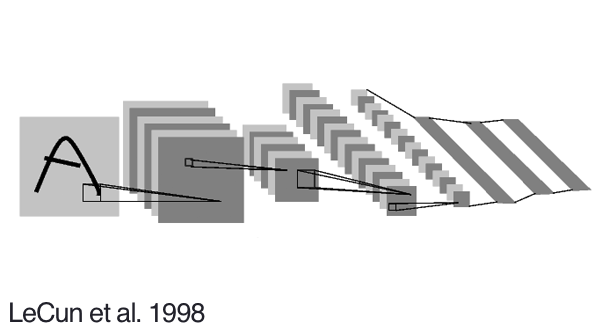
\includegraphics[width=\textwidth]{./imagenes/lenet.png}
\end{figure}

\subsection{Convolutional Layer}

En estas capas se aplica una operación de convolución a la entrada y el resultado es pasado a la siguiente capa. La operación de convolución emula la respuesta de una neurona individual ante un estímulo visual. Los parámetros de una red convolucional se componen de una serie de filtros que se aprenden. Cada filtro es pequeño, pero se extiende a lo largo de toda la profundidad de la entrada, en este caso una imagen. Esto quiere decir que si el filtro es 5x5 y la imagen es de 50x50, iremos pasando el filtro por cuadrados de 5x5 de la imagen hasta haberla recorrido en su totalidad.\\

Entonces, la red aprenderá filtros que se activen cuando vean cierto tipo de característica, como por ejemplo una esquina. Tendremos un filtro por neurona, por lo que habrá tantos filtros como neuronas tenga la capa de convolución.\\

\begin{figure}[H]
	\centering
	\caption{Ejemplo de filtros aprendidos por parte de Krizhevsky et al.}
    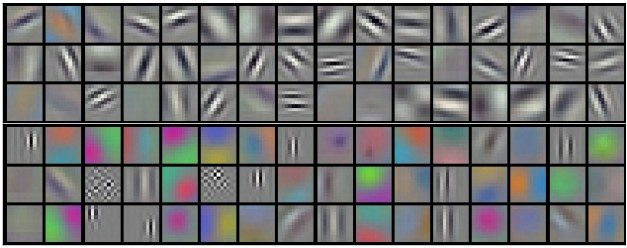
\includegraphics[width=\textwidth]{./imagenes//weights.jpeg}
\end{figure}

\subsection{Pooling Layer}
Es bastante normal insertar una capa de pooling entre sucesivas capas convolucionales. La función de una capa de pooling es reducir progresivamente el tamaño espacial de la representación para reducir la cantidad de parámetros y la computación en la red, y ayuda también para el control del overfitting. La capa de pooling opera independientemente en cada porción de profundidad de la entrada y le cambia el tamaño espacialmente, usando la operación de MAX. Lo que esto implica es que cada vez que aplicamos una capa de pooling, vamos reduciendo el tamaño espacial de la imagen.\\

Un ejemplo. Si tenemos una imagen de 224x224 y utilizamos una capa de pooling de 2x2, a la salida de esa capa, nuestra imagen, o mejor dicho la representación de la misma dentro de la red, tendrá un tamaño de 112x112, ya que la hemos reducido a la mitad con la operación de pool. Con la operación de MAX, lo que hacemos es que nos quedamos con el valor del máximo dentro de un grupo de píxeles.\\

\begin{figure}[H]
	\centering
	\caption{Ejemplo de capa de pool.}
    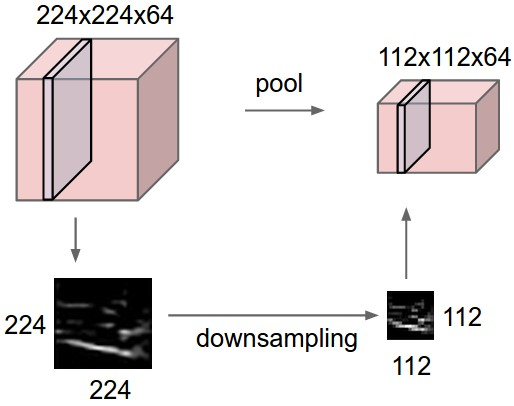
\includegraphics[width=\textwidth]{./imagenes/pool.jpeg}
\end{figure}
\begin{figure}[H]
	\centering
	\caption{Ejemplo de la operación maxpool.}
    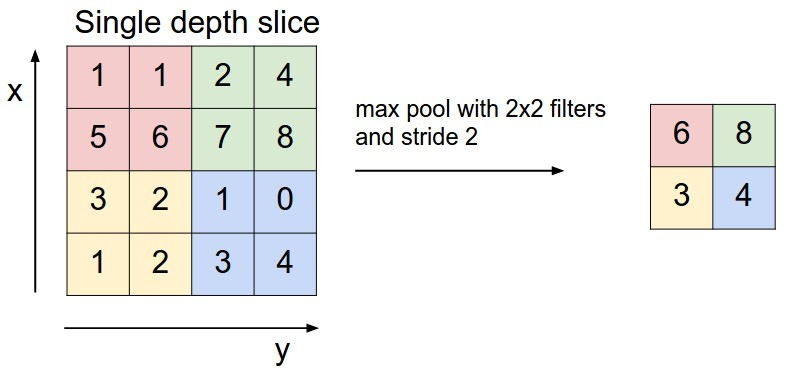
\includegraphics[width=\textwidth]{./imagenes/maxpool.jpeg}
\end{figure}

\subsection{Funciones de activación}

Como se ha explicado en la sección de las redes neuronales \ref{RedesNeuronales}, podemos tener distintas funciones de activación. Estas, definen la salida de la neurona dependiendo de cuál ha sido la entrada.\\

En nuestro caso usamos dos funciones de activación. Una es la función conocida como ReLU(Rectified Linear Unit) y la otra es la función conocida como Softmax.
\begin{figure}[H]
	\centering
	\caption{Función de activación Softmax}
	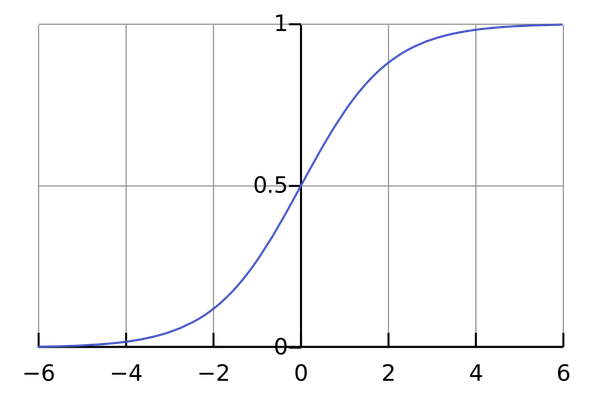
\includegraphics[height=300px,width=400px]{./imagenes/softmax.png}
\end{figure}
\newpage
\begin{figure}[H]
	\centering
	\caption{Función de activación ReLU}
	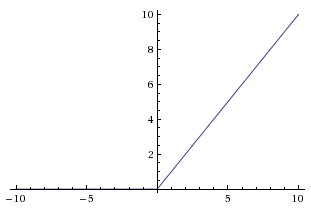
\includegraphics[height=300px,width=400px]{./imagenes/relu.jpg}
\end{figure}

La función de activación Softmax es la que se utilizará a la salida de la CNN para que nos de un valor de predicción. En el caso de que este valor sea 0, se clasificará la imagen como AD, y en el caso de que sea 1 se clasificará como Normal.\\

\section{Métodos de validación de modelos}

Para la validación del modelo empleado se han utilizado dos métodos, los cuáles son \textit{K-Fold cross-validation} y el \textit{Leave-one-out cross-validation}, que a continuación serán explicados brevemente.\\

\subsection{K-Fold Cross-Validation}

En el \textit{K-Fold Cross-Validation} se realiza una partición aleatoria del conjunto de datos en K partes. Entonces, se utilizará uno de estos subconjuntos para \textit{test} y los k-1 subconjuntos restantes se utilizarán para \textit{training}. Esto se repite K veces, sin repetir un subconjunto en \textit{test}. Entonces, se obtiene una media de los resultados en \textit{test} y con esto podemos hacernos una idea de como funciona nuestro modelo y de si generalizará bien. Esto incrementa el tiempo de entrenamiento y comprobación, por lo que no es un método muy usado en los los conjuntos de datos cuyo tamaño es muy grande, pero es de gran ayuda en conjuntos de datos más pequeños lo que nos permite validar mejor como será la generalización del modelo.\\

\begin{figure}[H]
	\centering
	\caption{Ejemplo de Cross Validation con K=4 \cite{k-fold}}
	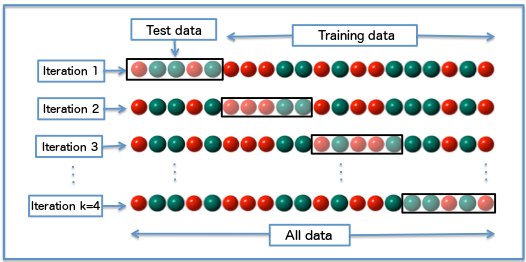
\includegraphics[width=\textwidth]{./imagenes/K-fold.jpg}
\end{figure}

\subsection{Leave-one-out Cross-Validation}
Este método podría ser un tipo de \textit{K-Fold cross-validation} en el que K es igual al número de elementos dentro del conjunto de datos. Esto implica que el tiempo de validación sea muy alto, ya que vamos a realidar K entrenamientos y K evaluaciones, pero es un método muy robusto para la validación del modelo.

\begin{figure}[H]
	\centering
	\caption{Ejemplo de  \textit{Leave one out Cross Validation} \cite{LOO}}
	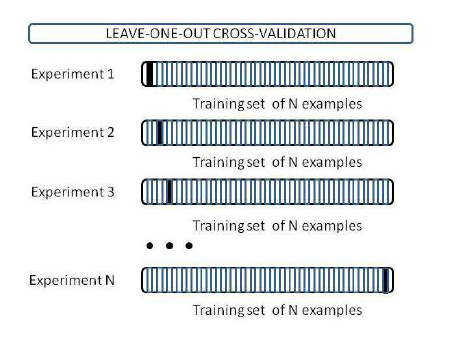
\includegraphics[width=\textwidth]{./imagenes/LOO.png}
\end{figure}

\mychapter{4}{Análisis del diagnóstico de la enfermedad de Alzheimer}

\section{Análisis de estudios médicos}

En la última década, el uso de neuroimágenes para el diagnóstico de un paciente ha crecido exponencialmente. Hace solo 10 años los parámetros de la \textit{American Academy of Neurology} indicaban que las tomografías computarizada (TC/CT) y las resonancias magnéticas (MR) eran opciones de examinación opcionales. Sin embargo, se tienen bastantes pruebas para afirmar que los análisis de cambios estructurales y funcionales pueden tener un impacto en el proceso de tratamiento de un paciente. \cite{SCHELTENS200213}.\\

Actualmente, las recomendaciones de la \textit{American Acafemy of Neurology} para el estudio de la demencia incluyen una examinación por imagen, una tomografía axial computarizada (TAC/CAT) o un MRI craneal. Aunque el TAC es una prueba más rápida, barata y accesible, el MRI tiene unas ventajas las cuáles son una mejor resolución y contraste entre los tejidos y puede detectar anormalidades focales existentes y no utilizada radiaciones ionizantes. Además, el MRI puede llegar a ser la técnica elegida en los estudios relegando al TAC en casos en los que las causas secundarias de la demencia deben ser descartadas rápido. En las Figura \ref{mriscan} y Figura \ref{catscan} podemos observar un ejemplo de una imagen obtenida por MRI y otra por TAC.\\

La perdida neuronal y consecuentemente la atrofia del cerebro causa un ensanchamiento de los surcos, un estrechamiento de los giros cerebrales y una dilatación de los ventrículos con una reducción significativa del peso del cerebro. En años recientes, se han identificado diferentes distribuciones de atrofia dependiendo del tipo de demencia. Para el alzheimer, los efectos de la atrofia afectan al promedio del lóbulo temporal. De tofas formas, las medidas de la atrofia en general no parecen que sean útiles para el diagnóstico del Alzheimer ya que la mayoría de enfermedades neurodegenerativas causan una atrofia global similar.

\begin{figure}[H]
	\label{mriscan}
	\caption{Ejemplo de imagen obtenida por MRI}
	\centering
	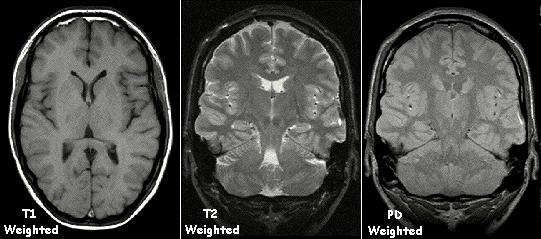
\includegraphics[width=350px]{imagenes/mriscanexample.jpg}
\end{figure}
\begin{figure}[H]
	\label{catscan}
	\caption{Ejemplo de imagen obtenida por CAT}
	\centering
	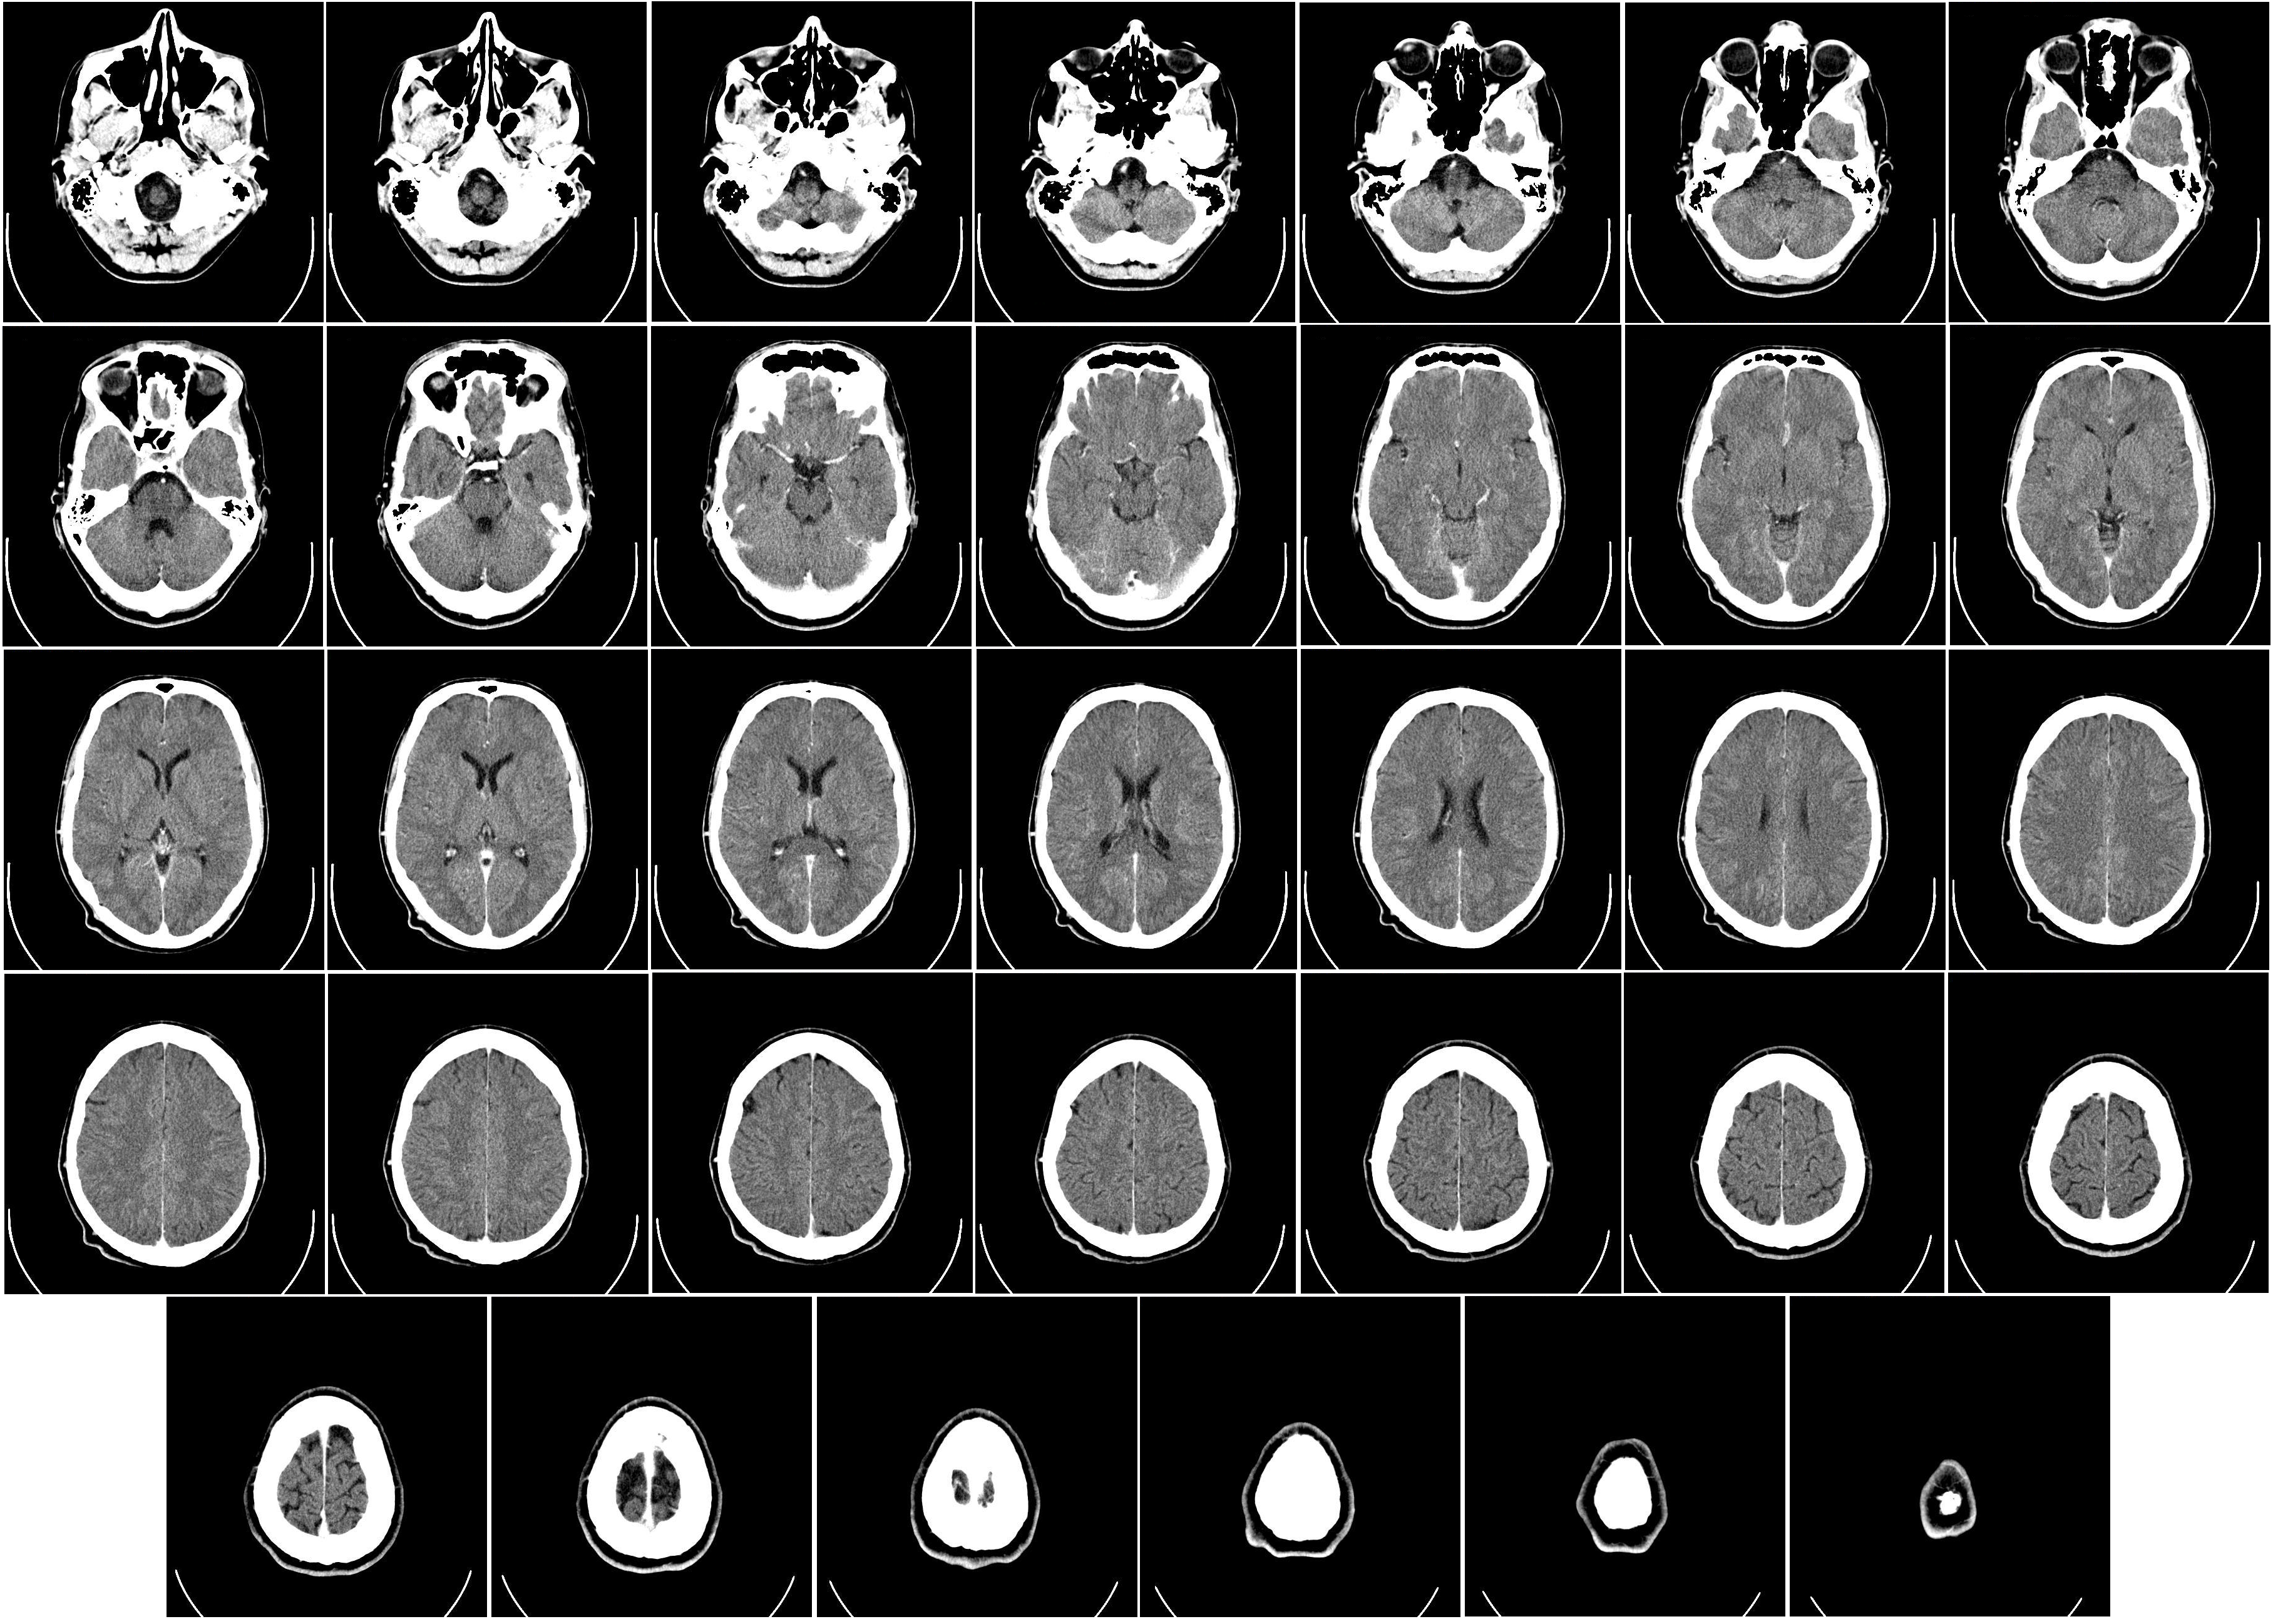
\includegraphics[width=350px]{imagenes/catimage.png}
\end{figure}
\newpage

En la siguiente tomografía del cerebro de un paciente se puede observar la perdida de la función del lóbulo temporal:

\begin{figure}[H]
	\label{perdidaLT}
	\caption{Tomografía del cerebro de un paciente con alzheimer mostrando pérdida de la función en el lóbulo temporal.}
	\centering
	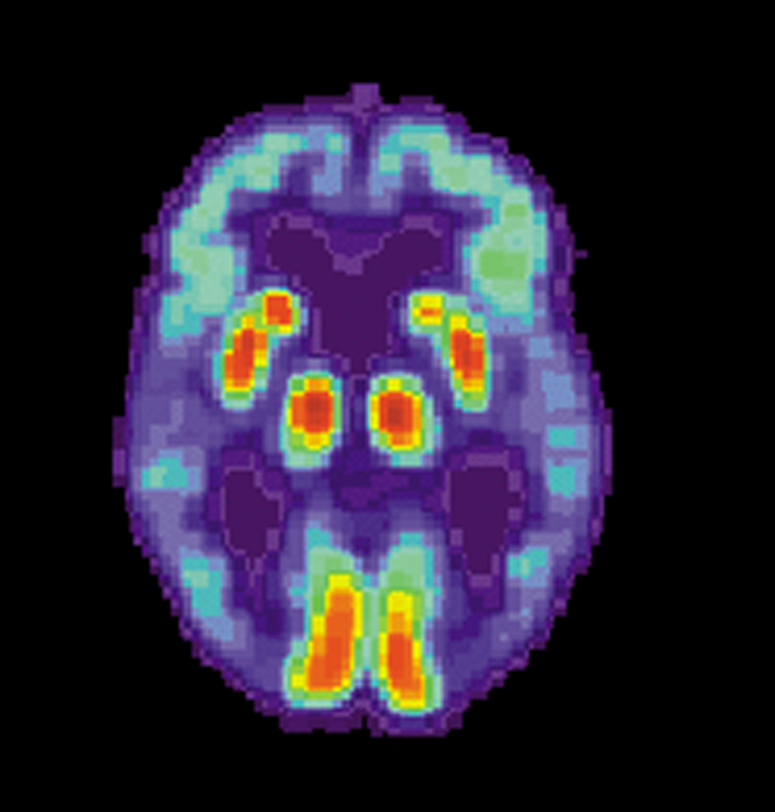
\includegraphics[height=200px,width=200px]{imagenes/perdidaLT.jpg}
\end{figure}


Muchos estudios se han enfocado en cuantificar cuál es la cantidad de atrofia en el lóbulo temporal, e incluso existen escalas para cuantificar cuál es el grado de atrofia, las cuáles son rápidas y fáciles de usar. En la última década, también se han desarrollado métodos automáticos para medir el grado medio de atrofia en el lóbulo temporal \cite{Hattori2007}, y esto se ha utilizado para la predicción de pacientes que padecen la enfermedad \cite{Visser491}.\\

En paralelo, también se ha observado que los pacientes de Alzheimer una notable atrofia en regiones posteriores conocida como atrofia cortical. Esto parece ser característico, pero no exclusivo, de la enfermedad de Alzheimer. Es por ello, que en la última época, se han intentado proponer escalas visuales para cuantificar el grado de atrofia cortical \cite{Koedam2011}.\\

Recientemente también se han realizado estudios sobre la diferencia de la atrofia en el hipocampo y cortical hipo-metabolismo de personas que no padecen la enfermedad y las que sí, pudiendo llevar a mejores diagnósticos. \cite{Chung2017}.\\

También se ha podido observar que la atrofia cerebral comienza años antes del diagnóstico del Alzheimer. De hecho, la atrofia del hipocampo aparece en pacientes con riesgo de padecer Alzheimer años antes de que los síntomas comiencen., como se puede observar en \cite{fox1996presymptomatic}.\\

\section{Análisis de estudios basados en computación}

Por otra parte, el estudio de la enfermedad basándose en el uso del análisis de las imágenes MRI mediante algoritmos de \textit{Machine Learning} es un campo que en la última década ha cobrado mucha fuerza a la hora del diagnóstico de la enfermedad. En \cite{CHAPLOT200686} podemos observar el uso ondas y características de las imágenes para entrenar un algoritmo SVM  y también el uso de redes neuronales con mapas auto organizados de características (SOM) con el fin de clasificar entre cerebros normales o anormales, obteniendo unos buenos resultados de \textit{accuracy}.\\

Estudios siguientes continuaban la misma línea de trabajo, usando como características las ondas cerebrales y luego utilizando algún algoritmo de \textit{Machine Learning} como clasificador. Además, también se incluyeron métodos como el PCA( \textit{Principal Component Analysis}) para reducir el tamaño dimensional de los datos. \cite{Lee:2009:CMF:1697406.1697471}\\

Dentro de nuestra propia universidad, tenemos trabajos que demuestran que el uso de SVM con las apropiadas características de ondas y de las propias imágenes además d el uso del PCA para la reducción de la dimensión, permite obtener unos buenos resultados a la hora de la clasificación, como se puede comprobar en \cite{jaramillo}.\\

Hoy en día, con los avances que se han producido con la introducción de nuevos algoritmos de Deep Learning además del avance en las técnicas de adquisición de imágenes, muchos estudios han intentado utilizar estas técnicas para mejorar la clasificación de los pacientes.\\

La mayoría de estos estudios hacen uso de redes convolucionales con muchas capas para el entrenamiento y aprendizaje de filtros que puedan ser útiles a la hora de clasificar a los pacientes. Entre ellos cabe destacar el siguiente estudio \cite{residualVGG}, en el que se utilizaban imágenes MRI en 3D junto con redes convolucionales tridimensionales para el aprendizaje y clasificación de pacientes. En este se obtienen unos resultados muy destacables, partiendo de una base de datos muy reducida.\\

También se pueden encontrar estudios en los cuáles el uso de redes convolucionales junto con el uso de \textit{autoencoders}, se obtienen buenos resultados en el \textit{accuracy} a la hora de la clasificación de los pacientes, como se puede observar en \cite{DBLP:journals/corr/Hosseini-AslKE16}.\\

Como se puede observar, la mayoría de estudios realizados hacen usos de redes convolucionales en tres dimensiones, lo que produce que se necesite mucha capacidad de computación y tiempo para obtener los resultados del entrenamiento. Este es un campo en el que aún queda mucho desarrollo, sobre todo para llegar a unas técnicas que se pudiesen implantar como ayuda a la toma de decisión de un médico en caso de diagnóstico.\\

\mychapter{5}{Análisis y Desarrollo Experimental}

En este capítulo voy a hacer una recapitulación de la estructura y desarrollo de los experimentos que se han llevado a cabo para la realización de este TFG, además de una breve exlicación de las distintas herramientas que se han utilizado para ello.\\

\section{Máquinas en las que se han realizado los experimentos}

Las dos máquinas principales en las que se han realizado los experimentos han sido las siguientes:
\begin{itemize}
	\item \textbf{MacBook Air 2016}: \textit{Procesador}, 1,6 GHz Intel Core i5. \textit{Memoria},8 GB 1600 MHz DDR3. Principalmente utilizado para el procesamiento de las imágenes NIFTI.
	\item \textbf{Servidor}: \textit{Procesadores}, 2 Intel(R) Xeon(R) CPU   E5645  @ 2.40GHz. \textit{GPU}, 2 Tesla C2050 / C2075. Utilizada para la realización de los experimentos.
\end{itemize}
\section{Herramientas utilizadas}

En primer lugar, quiero citar cuáles han sido las herramientas utilizadas para la realización de este trabajo.\\
\subsection{Librerías para trabajar con técnicas de Deep Learning }

Actualmente debido a los grandes avances que se han conseguido en ciertos campos con el uso de técnicas de Deep Learning. el número de librerías dedicadas a facilitar la realización de experimentos con este tipo de técnicas ha crecido a una gran velocidad, dejándonos muchas opciones donde elegir.\\

Existe un abanico muy amplio de librerías donde elegir, entre ellas hay librerías que llevan más tiempo como por ejemplo \textbf{Caffe}\cite{Caffe} o \textbf{Theano}\cite{Theano} y otras cuyo tiempo de vida es menor. En este último grupo encontramos una librería que en los últimos años ha tenido mucha repercusión, la cuál es \textbf{Tensorflow}\cite{Tensorflow}. Su gran crecimiento puede deberse a varios factores, entre ellos su rapidez (dentro de lo posible) en tiempos de computación,y que viene de la mano de Google.\\

La mayoría de estas librerías requiere mucho conocimiento técnico de lo que se está haciendo y controlar a mano muchos parámetros que pueden suponernos un retraso a la hora de la realización de los experimentos, debido a necesitar tiempo para arreglar fallos dentro del código.\\

Es por estos motivos por los que François Chollet, un trabajador de Google, creó la \textit{high-level API} \textbf{Keras}\cite{keras}. Keras, es una librería que nos sirve como capa para la utilización tanto de Tensorflow como Theano. Nos permite, por ejemplo, métodos automáticos para el entrenamiento utilizando un número fijado de \textit{batch}, mientras que en Tensorflow o Theano tendríamos que programar esto a mano. Este tipo de ayudas permite que el tiempo que se requiere desde el momento en el que comienzas a programar un experimento hasta el fin de su ejecución sea el más rápido posible y lo más ausente de fallos.\\

Es por estas, y más razones, que se ha decido utilizar \textbf{Keras} como librería para trabajar con técnicas de Deep Learning.\\
\begin{figure}[H]
	\label{figure1}
	\centering
	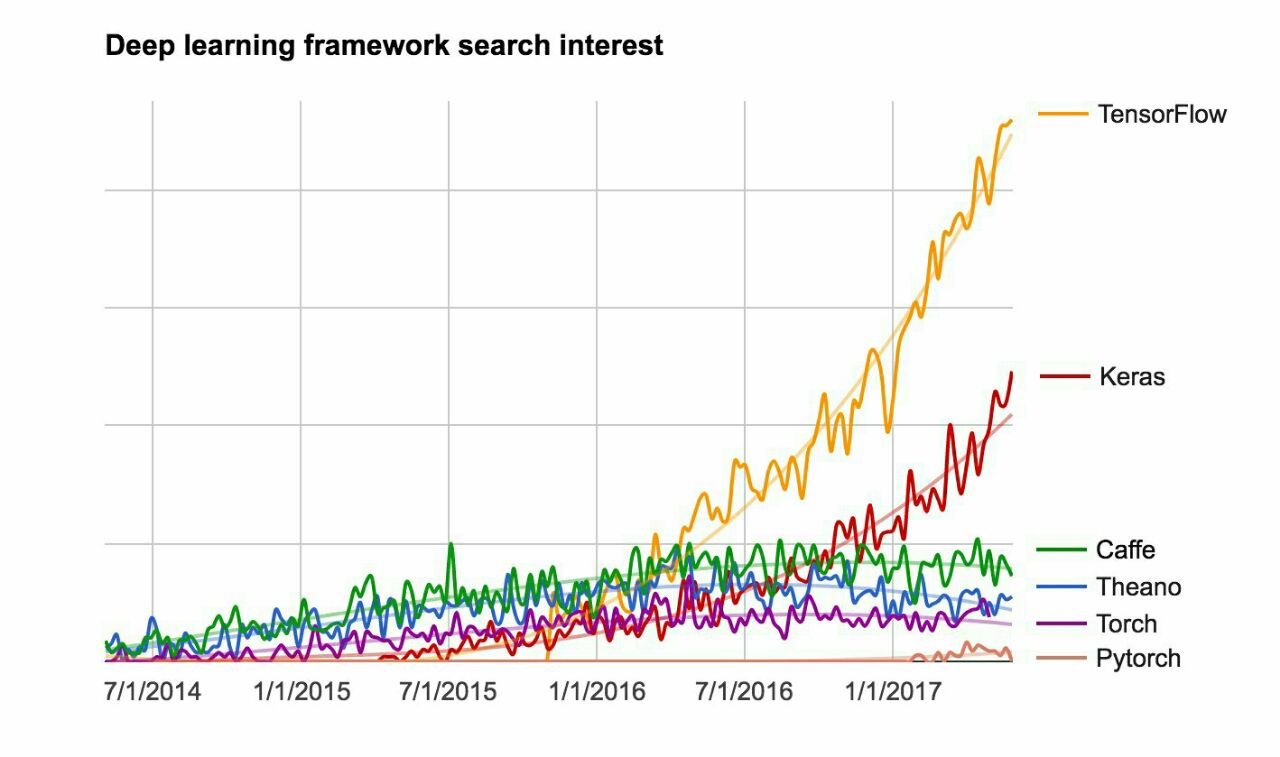
\includegraphics[width=350px]{imagenes/dlsearch.jpg}
	\caption{Interés de búsqueda de Frameworks de Deep Learning. Fuente: François Chollet}
\end{figure}

\begin{figure}[H]
	\label{figure1}
	\centering
	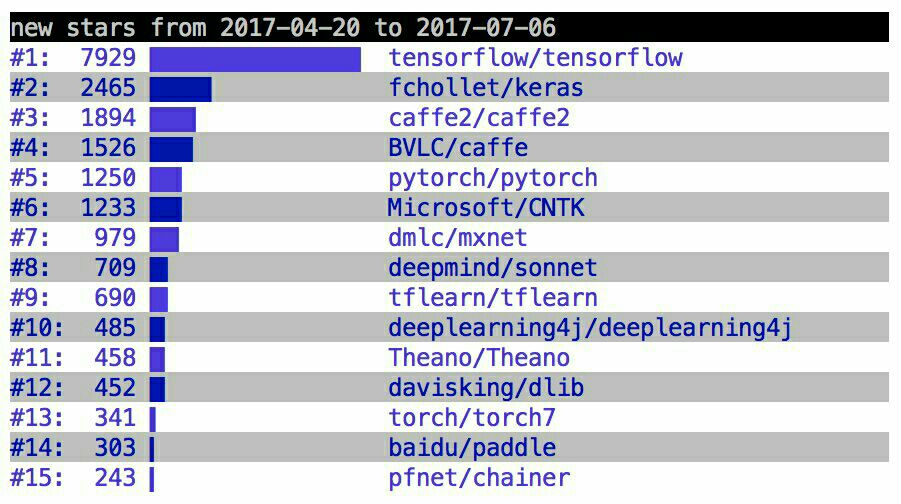
\includegraphics[width=\textwidth]{imagenes/dlstars.jpg}
	\caption{Stars a repositorios de Github. Fuente: François Chollet}
\end{figure}

\subsection{Librería para trabajar con las imágenes en formato NIFTI}
\label{nibabel}
Para poder trabajar con redes convolucionales en 2 dimensiones, debido a que la capacidad de computación requerida para trabajar con las imágenes en 3D no era posible, se requería una librería con la que poder obtener las capas del cerebro que nosotros quisiésemos y luego guardarlas en un formato con el que Keras pudiese tratar.\\
Para ello, se utilizó la librería para Python \textbf{Nibabel}\cite{Nibabel}. Esta librería nos permite obtener toda la información de un archivo NIFTI y poder coger el \textbf{slice} que queramos.\\
\section{Procesamiento de las imágenes NIFTI}
\label{procesamiento-imagenes}
En nuestro caso, se requería previamente obtener imágenes 2D a partir de laos archivos NIFTI. Esto era necesario a la hora de poder tratar estas imágenes con Keras, para la realización de los experimentos.Para ello, se creó un script llamado \textit{create\_slices.py}.\\

Con este script lo que se consigue es la lectura de todos los archivos NIFTI, obteniéndose las capas desde la 10 a la 100 de 5 en 5, y guardándose ordenadamente en una nueva carpeta correspondiente a cada capa, obteniendo 19 carpetas distintas.\\

Se guardan en esta estructura para luego poder leerlos ordenadamente y obtener resultados sobre cada slice del cerebro. Con esto se nos permitirá determinar cuál es la capa del
cerebro que mejor resultados nos da.\\
\section{Arquitectura de la CNN  \ref{CNN}}

Esta es una decisión muy importante a la hora de la realización del TFG. Para ello se revisó la bibliografía más reciente, para partir de una base sólida a la hora de la elección del modelo. En la revisión bibliográfica podemos encontrar estudios como \cite{residualVGG} y \cite{SarrafT16}.\\

Por parecernos más concluyentes los resultados de \cite{residualVGG} debido a la metodología de separación de pacientes que ellos utilizaban, se decidió utilizar la primera arquitectura que ellos introducen, basada en la arquitectura \textbf{VGG} \cite{SimonyanZ14a}.\\

La arquitectura podemos observarla en la Figura \ref{arquitectura}. En nuestro caso, se ha modificado para que sea una red que acepte entradas 2D en lugar de 3D.\\

En el artículo \cite{residualVGG} también se prueba otro tipo de arquitectura, un tipo de arquitectura residual. Pero en los resultados no se encuentra una mejora sustancial como para aplicar una arquitectura más compleja, y que requiera más tiempo de computación.\\
\section{Experimentos}

En esta sección, se irán explicando los distintos experimentos que se han llevado a cabo para el estudio de métodos para la clasificación de las imágenes en 2D y cuál sería la mejor estrategia para el análisis de las mismas, eligiendo la capa del cerebro más significativa para la clasificación.\\
\subsection{Parámetros comunes a todos los experimentos}

Hay unos parámetros comunes que se han utilizado para todos los experimentos, los cuáles se relatan a continuación.\\

Con respecto a la arquitectura, se ha utilizado como función de \textit{loss} la función \textbf{categorical cross-entropy} y un \textit{learnig rate} de \textbf{$27\times 10^{-6}$}.\\

Además, en cuanto al entrenamiento se refiere, se ha utilizado un número de \textit{epochs} igual a 70 y un \textit{batch size} de 5.\\
\subsection{Experimentos previos a los tres experimentos finales}

Al inicio comenzamos trabajando con una sola capa de todas las imágenes y se decidió utilizar la capa media del cerebro. En nuestro caso, al ser las imágenes de \textbf{110x110}. Como tenemos un conjunto de datos reducido, ya que solo disponemos de 389 imágenes y este número en términos de usar técnicas de Deep Learning es tener un conjunto de datos muy pequeño, decidimos usar técnicas de validación para poder determinar si los resultados obtenidos eran significativos o no. Para intentar emular los resultados del artículo \cite{residualVGG} previamente citado, se redujo el conjunto de datos al utilizar solo una imagen por paciente, ya que hay pacientes de los cuáles disponemos más de una imagen de distinto período temporal, dejando el conjunto de datos a una cantidad de 131 imágenes. Para ello se implementó un \textit{5-Fold Cross Validation}, ya que es lo que se utilizó en \cite{residualVGG} y además nos da una robustez en los resultados.\\

Viendo el desempeño que había tenido con el conjunto reducido se decidió comprobar si aumentando el número de imágenes se obtendrían mejores resultados. Esto quiere decir, utilizando todas las imágenes de los pacientes, pero siempre comprobando que no ocurra el caso en que dos imágenes distintas de un paciente se encuentre en \textit{train} y en \textit{test} al mismo tiempo. Para ello se hizo una separación manual de las imágenes en 5 \textit{folds} para la realización al igual que anteriormente de un \textit{5-fold Cross Validation}, siempre respetando la restricción anteriormente explicada y se obtuvo una mejora en los resultados.\\

En este momento, se pensó que quizá con otras capas se podrían llegar a mejores resultados, porque la red en esas imágenes aprendiese unos mejores filtros. Es por esto que se decidió utilizar otras capas para comprobar si existían diferencias.\\

Viendo que los resultados variaban según la capa que utilizases, decidimos responder a la pregunta, ¿cuál será la capa que mejor rendimiento nos dé a la hora de clasificar entre pacientes normales y pacientes con Alzheimer?. Con esto habríamos determinado que se puede hacer una clasificación de estos pacientes con CNN y que, además, hay ciertas capas dentro de una imagen tridimensional que nos ayudan a clasificar mejor a un paciente.\\

Como último dato, decir que también se aplicó otra alternativa para ver si había una correlación entre las imágenes de los pacientes o eran muy diferentes unas y otras. Se utilizó un \textit{5-Fold Cross Validation} sin asegurarse de que no se repetían distintas imágenes de los pacientes en distintos conjuntos, obteniendo resultados formidables. Esto no sirve sino para reforzar la idea de que no podemos usar imágenes del mismo paciente en distintos conjuntos, ya que puede llevar a la filtración de características que hagan más fácil la tarea de la red a la hora de clasificar.\\

\subsection{Experimento 1: Leaving-one-out Cross Validation con todas las imágenes}
\label{exp1}
El primer experimento a realizar se usó para confirmar la teoría de que hay filtración de información entre imágenes, junto con los resultados de experimento 2. En este caso, no se realizó ninguna separación de las imágenes de los pacientes, sino que se trataron como si todas fuesen imágenes distintas.\\

Es necesario añadir que el tiempo de ejecución de este experimento fue de alrededor de unas 28 horas, ya que la técnica de validación de \textit{LOO Cross-Validation} es muy demandante en cuanto a tiempo se refiere. A continuación, con el segundo experimento se iba a comprobar si de verdad existía una filtración de información entre imágenes del mismo paciente.\\
\newpage
\begin{figure}[H]
	\centering
	\caption{Arquitectura utilizada basada en la arquitectura VGG \cite{SimonyanZ14a} del artículo \cite{residualVGG}}
	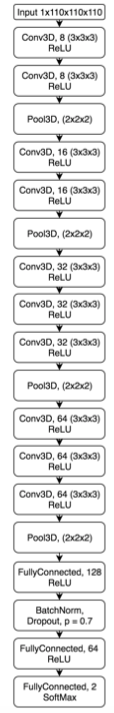
\includegraphics[height=\textheight]{imagenes/model.png}
	\label{arquitectura}
\end{figure}

\subsection{Experimento 2: Leaving-one-out Cross Validation por paciente}
\label{exp2}
Con este experimento, lo que se intentaba era comprobar si de verdad había una filtración de información entre las imágenes de los pacientes usando un método de validación más robusto como es el \textit{LOO Cross-Validation}.\\

Para ello lo que se realizó fue una implementación especial del algoritmo de \textit{LOO Cross-Validation} en el que en lugar de sacar en cada iteración un elemento al conjunto de \textit{test}, se meten en \textit{test} todas las imágenes que pertenece al mismo paciente paciente, gracias a un vector que contiene el número de identificación del paciente. Además, se lleva un registro de los pacientes que ya se han introducido en \textit{test} para que cuando se continúe con el entrenamiento y nos encontramos con otra imagen del mismo paciente no se vuelva a realizar lo mismo que se ha realizado previamente.\\
\subsection{Experimento 3:  5-Fold Cross Validation para ver cuál es la mejor capa}

Una vez realizados los experimentos previos decidimos responder a la pregunta, ¿cuál será la capa del cerebro con la que se obtienen mejores resultados?. Por lo tanto, se realizó un \textit{5-Fold Cross Validation} para comprobar cuál es la capa que mayor rendimiento obtiene en cuanto a \textit{accuracy} en el conjunto de \textit{test}.\\

La separación de los pacientes se realizó manualmente, para asegurarnos de que no hubiese imágenes del mismo paciente en distintos conjuntos. Esto nos dejó con 4 conjuntos compuestos pro 77 imágenes y el último compuesto por 76 imágenes.
\mychapter{6}{Base de datos empleada}

La base de datos empleada ha sido una de las bases de datos más utilizadas y trabajadas para el estudio del Alzheimer, que es la base de datos conocida como \textbf{ADNI (Alzheimer’s Disease Neuroimaging Initiative)}. La base de datos pone a disposición datos clínicos de pacientes tales como: imágenes MRI y PET, informes genéticos, test cognitivos y biomarcadores de la sangre. Estos pacientes pertenecen a un grupo de estudio voluntario realizado en Norte América dentro de los cuales se incluye pacientes que padecen de Alzheimer, pacientes que muestran un deterioro cognitivo leve y grupos de control, es decir, sujetos sanos.\\

El estudio de ADNI ha tenido tres fases: ADNI1, ADNI GO y ADNI2. En cada una de ellas se incorporaban pacientes nuevos para su evaluación médica. Esta evaluación y seguimiento médico se usaban para detectar cualquier patología de Alzheimer en los pacientes.\\

En nuestro caso se ha utilizado un subconjunto dentro de ADNI en el cuál se había realizado cierto post-procesamiento de las imágenes obtenidas que será explicado a continuación.\\
\section{Post procesamiento}

El post-procesamiento está compuesto por los siguientes pasos:
\begin{itemize}
	\item \textbf{\textit{Spatially Normalized}:} Con este paso lo que se consigue es que un mismo pixel corresponda a la misma posición en dos imágenes cerebrales distintas.
	\item \textbf{\textit{Masked}:} Con este paso conseguimos aislar la masa cerebral eliminando el cráneo. 
	\item \textbf{\textit{N3 Correction}:} Con este paso realizamos una corrección de la intensidad en la imagen.
\end{itemize}
\label{postproces}

Esto permite que tengamos unas imágenes escaladas, centradas y con solo la masa cerebral, lo que nos puede ayudar a que la red aprenda mejores filtros para realizar la clasificación de las imágenes.\\
\begin{figure}[H]
	\centering
	\caption{Ejemplo de una imagen con el post-procesamiento relatado en \ref{postproces}}
	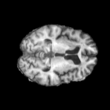
\includegraphics[height=300px,width=300px]{./imagenes/ejemplo_imagen.png}
\end{figure}

\section{Software de visualización de las imágenes}

Para la visualización de estas imágenes podemos hacer uso de varias herramientas. La utilizada para la visualización de las imágenes en formato \textit{NIFTI} ha sido el software \textbf{MRIcron}\cite{mricron}. Este software nos permite visualizar los diferentes cortes cerebrales (coronal, sagital y axial) que están contenidos en el archivo NIFTI.\\

\begin{figure}[H]
	\centering
	\caption{Ejemplo de visualización de una imagen con el software MRIcron \cite{mricron}}
	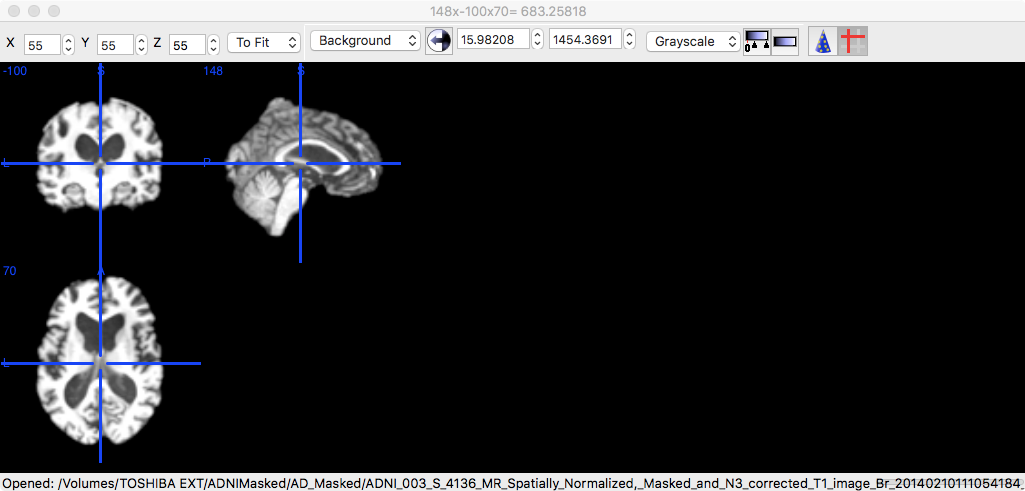
\includegraphics[width=\textwidth]{./imagenes/ejemplomricron.png}
\end{figure}

\section{Separación de las imágenes por tipos}

En cuanto a la clasificación de las imágenes, anteriormente cada imagen tenía asociado un archivo \textit{XML} donde venía resumida la información del paciente y a qué tipo de grupo pertenecía. Pero durante este año se ha llevado a cabo una reorganización de la base de datos por lo que ahora, para la separación de los pacientes según el tipo, se utiliza la búsqueda avanzada señalando en una casilla que tipo de pacientes quieres buscar. Así también se han obtenido los imágenes de los pacientes a las que se le había aplicado el post-procesamiento previamente explicado.
\mychapter{7}{Resultados}

\section{Resultados de experimentos previos a los tres experimentos finales}
\label{experimentosprevios-resultados}
En cuánto a los experimentos previos tenemos unos resultados que son los que han ido desencadenando como ha continuado la realización de este trabajo. En cuanto a los resultados del primer experimento realizado, en el cuál se intentaban imitar los resultados obtenidos en \cite{residualVGG} utilizando solo la capa 55, son muy bajos, obteniendo una media del \textit{accuracy} en los conjuntos de \textit{test} de \textbf{43'5043\%}.\\

Si pasamos al segundo experimento previo, en el cuál se intentaba comprobar si teniendo más imágenes pero guardando una separación entre las imágenes de un mismo paciente, podemos observar que se obtiene una mejora en los resultados, con una media del \textit{accuracy} en los conjuntos de \textit{test} de \textbf{ 50'2358\%}, aunque no muy superior al anterior experimento.\\

A continuación, al probar si con capas distintas los resultados variaban, se probó con la capa 45 y al 65 obteniendo resultados más favorables con \textbf{67'9802\%} y \textbf{52'2556\%} respectivamente.\\

Por último, se realizó un experimento para observar si podía existir filtración de información entre imágenes distintas del mismo paciente. Al realizar este experimento, los resultados fueron magníficos obteniendo un \textbf{92\%} de \textit{accuracy} de media en los conjuntos de \textit{test} usando la capa 45 de las imágenes.\\

A continuación se puede observar una tabla con un compendio de los resultados previos y una gráfica con los mismos:
\begin{table}[H]
	\centering
	\label{tablarendimientos}
	\caption{Tabla con los resultados obtenidos en distintos experimentos}
	\begin{tabular}{|l|l|}
		\hline
		\begin{tabular}[c]{@{}l@{}}5-Fold CV Conjunto Reducido\\                   Capa 55\end{tabular}       & 43'5043\% \\ \hline
		\begin{tabular}[c]{@{}l@{}}5-Fold CV Conjunto Completo\\                   Capa 55\end{tabular}       & 50'2358\% \\ \hline
		\begin{tabular}[c]{@{}l@{}}5-Fold CV Conjunto Completo\\                   Capa 45\end{tabular}       & 67'9802\% \\ \hline
		\begin{tabular}[c]{@{}l@{}}5-Fold CV Conjunto Completo\\                   Capa 65\end{tabular}       & 52'2556\% \\ \hline
		\begin{tabular}[c]{@{}l@{}}5-Fold CV Conjunto Completo\\ Repitiendo pacientes capa 45\end{tabular} & 92\%       \\ \hline
	\end{tabular}
\end{table}
\begin{figure}[H]
	\label{figure1}
	\caption{Rendimiento en los distintos experimentos, el orden es el mismo que en la tabla \ref{tablarendimientos}}
	\centering
	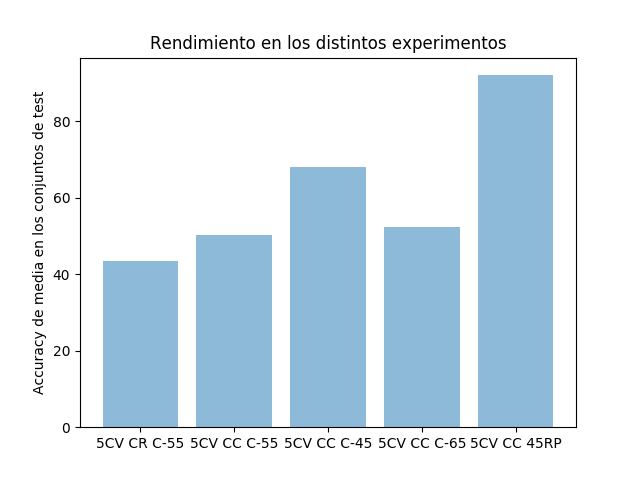
\includegraphics[width=\textwidth]{imagenes/rendimiento_experimentos.png}
\end{figure}
\section{Resultados Experimento 1: Leaving-one-out Cross-Validation con todas las imágenes}
\label{experimento1-resultados}
Como se esperaba, al no realizar una separación de imágenes y con la sospecha de que la filtración de información entre imágenes favorecía a su clasicación, los resultados de este experimento son muy buenos, obtenido un \textbf{77'6042\%} de \textit{accuracy} de media en los conjuntos de \textit{test}, utilizando la capa 45 del cerebro. Estos resultados no son nada significativos para el estudio, ya que se sabe que existe una filtración de información, por lo que solo sirven para confirmar esta teoría.\\
\section{Resultados Experimento 2: Leaving-one-out Cross-Validation por paciente}
\label{experimento2-resultados}
En este experimento se intenta comprobar si existía una filtración de información entre distintas imágenes del mismo paciente. Los resultados obtenidos dejaron relucir que si se produce una filtración de información entre las imágenes de los pacientes ya que se obtuvo un \textbf{60'5655\%} de \textit{accuracy} de media en los conjuntos de \textit{test}, muy inferior al que se obtuvo en el experimento 1 \ref{exp1}, en el cuál si se incluían imágenes distintas del mismo paciente en los conjuntos de \textit{train} y \textit{test}.\\
\section{Experimento 3:  5-Fold Cross Validation para ver cuál es la mejor capa}
\label{experimento3-resultados}
Para la realización del 3 experimento, se tomaron las capas desde la \textbf{10 a la 100} de 5 en 5. Los resultados de \textit{accuracy} de media en los conjuntos de \textit{test} en las distintas capas se pueden observar en la siguiente tabla \ref{tablaexperimento3}:\\
\begin{figure}[H]
	\label{figure1}
	\caption{Rendimiento de las distintas capas}
	\centering
	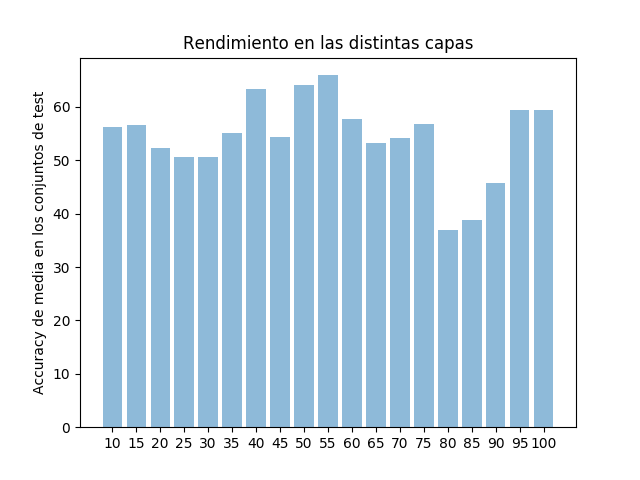
\includegraphics[height=200px,width=\textwidth]{imagenes/experimento3.png}
\end{figure}
\newpage
\begin{table}[H]
	\centering
	\label{tablaexperimento3}
		\caption{Tabla con los resultados obtenidos por las distintas capas}
	\begin{tabular}{|l|l|}
		\hline
		\begin{tabular}[c]{@{}l@{}}Nº Capa \ \end{tabular}       & Accuracy(\%) \\ \hline
		\begin{tabular}[c]{@{}l@{}}Capa 10\ \end{tabular}       & 56'326\% \\ \hline
		\begin{tabular}[c]{@{}l@{}}Capa 15 \end{tabular}       & 56'5619\% \\ \hline
		\begin{tabular}[c]{@{}l@{}}Capa 20 \end{tabular}       & 52'3479\% \\ \hline
		\begin{tabular}[c]{@{}l@{}}Capa 25 \end{tabular}       & 50'6972\% \\ \hline
		\begin{tabular}[c]{@{}l@{}}Capa 30 \end{tabular} & 50'6972\%       \\ \hline
		\begin{tabular}[c]{@{}l@{}}Capa 35 \end{tabular} & 55'1948\%       \\ \hline
		\begin{tabular}[c]{@{}l@{}}Capa 40 \end{tabular} & 63'2912\%       \\ \hline
		\begin{tabular}[c]{@{}l@{}}Capa 45 \end{tabular} & 54'3643\%       \\ \hline
		\begin{tabular}[c]{@{}l@{}}Capa 50 \end{tabular} & 64'1046\%       \\ \hline
		\begin{tabular}[c]{@{}l@{}}Capa 55 \end{tabular} & 65'9467\%       \\ \hline
		\begin{tabular}[c]{@{}l@{}}Capa 60 \end{tabular} & 57'7204\%       \\ \hline
		\begin{tabular}[c]{@{}l@{}}Capa 65 \end{tabular} & 53'3151\%       \\ \hline
		\begin{tabular}[c]{@{}l@{}}Capa 70 \end{tabular} & 54'149\%       \\ \hline
		\begin{tabular}[c]{@{}l@{}}Capa 75 \end{tabular} & 56'7601\%       \\ \hline
		\begin{tabular}[c]{@{}l@{}}Capa 80 \end{tabular} & 36'9139\%       \\ \hline
		\begin{tabular}[c]{@{}l@{}}Capa 85 \end{tabular} & 38'7526\%       \\ \hline
		\begin{tabular}[c]{@{}l@{}}Capa 90 \end{tabular} & 45'7758\%       \\ \hline
		\begin{tabular}[c]{@{}l@{}}Capa 95 \end{tabular} & 59'4532\%       \\ \hline
		\begin{tabular}[c]{@{}l@{}}Capa 100 \end{tabular} & 59'4532\%       \\ \hline
	\end{tabular}
\end{table}
\mychapter{8}{Conclusiones y trabajos futuros}

En este capítulo se va a hablar de las conclusiones que se pueden observar a partir de los resultados obtenidos en el capítulo anterior y trabajos futuros que se desearían realizar a partir de lo ya concluido con este trabajo.\\

\section{Conclusiones}

Con este trabajo se intentaban dar respuesta a varias cuestiones. Una sería si \textbf{se pueden obtener buenos resultados usando técnicas de \textit{Deep Learning} para la clasificación de imágenes de pacientes con Alzheimer y pacientes sin esta enfermedad usando imágenes en 2D}, al contrario que en estudios previos donde se utilizaban las imágenes en 3D \cite{residualVGG}.\\

Como se puedo observar en los experimentos previos \ref{experimentosprevios-resultados} y con el experimento 2 \ref{experimento2-resultados}, los resultados mejoran cuanto mayor es la base de datos que tenemos. Esto deja dilucidar que si aumentamos la base de datos cada vez con más imágenes se podrían obtener muy buenos resultados a la hora de la clasificación de pacientes que nos llegasen, pudiendo llegar a ser una herramienta de utilidad a la hora de que un médico pudiese hacer un diagnóstico a un paciente. Además, al tratarse de imágenes 2D en lugar de 3D, el tiempo para el entrenamiento y la capacidad de computación necesaria para el mismo o la predicción se reducen notablemente, dejando un camino abierto para que se pudiese realizar en un ordenador menos potente, lo cuál abriría más caminos para que se pudiese implantar un sistema así en un hospital.\\

La segunda cuestión a la que se intentaba dar respuesta era que, una vez visto que la clasificación de los pacientes con imágenes 2D es viable y se pueden observar mejoras, \textbf{cuál es la capa del cerebro con la que se debería hacer esta clasificación}. Para ello se preparó el experimento 3, y se pueden ver sus resultados en \ref{experimento3-resultados}. Con estos en mano podemos observar que las mejores capas para la clasificación son la \textbf{40,55,50}. Aun así, son un poco optimistas, ya que vimos en el experimento 2 \ref{experimento2-resultados} que nuestro techo de \textit{Accuracy} utilizando un método de validación muy robusto como es el \textit{LOO CV} era de un \textbf{60'5655\%}. Con estos resultados también hemos podido afirmar que hay unas capas que funcionan mejor que otras.\\

Además, como también hemos comprobado que hay una filtración de información entre distintas imágenes del mismo paciente con los resultados en \ref{experimentosprevios-resultados} y \ref{experimento1-resultados}, siempre tenemos que realizar una separación de los pacientes y esto se debería realizar también a la hora de que se implantase este procedimiento en un centro médico. \\

Esto por esto que los resultados \textbf{más significativos y en los que se basa este trabajo} son los obtenidos en los experimentos 2 \ref{experimento2-resultados} y 3 \ref{experimento3-resultados}.\\

Gracias a estos resultados podríamos afirmar que hay un futuro a la hora de realizar predicciones sin utilizar imágenes 3D, reduciendo los costes de computación y sin realizar un procesamiento de las imágenes muy costoso como se ha explicado en \ref{procesamiento-imagenes}, pero que se debe disponer de una mayor base de datos para que incrementemos la generalización de la red. Además, se ha confirmado que la estructura de la red utilizada en \cite{residualVGG} es útil también para la clasificación de imágenes 2D, obteniendo unos resultados aceptables en \ref{experimento2-resultados} y \ref{experimento3-resultados}.\\

Lo que también se puede afirmar es que un mayor número de imágenes de pacientes da lugar a unos mejores resultados, como se pudo observar en los experimentos previos que se realizaron \ref{experimentosprevios-resultados}. Esto indicaría que si se pudiese normalizar la base de datos actual y aplicarle el post procesamiento \ref{postproces} al que fue sometida la base de datos utilizada para este trabajo, se podrían obtener unos muy buenos resultados a la hora de la clasificación de los pacientes.\\

\section{Trabajos futuros}

En cuanto a los trabajos futuros a partir del actual, el principal sería continuar por la línea de comprobar si cuantas más imágenes mejores resultados. Actualmente solo se ha utilizado un subgrupo dentro de la base de datos donde se había aplicado el post procesamiento explicado en \ref{postproces}. Como continuación, nos gustaría aplicar el post procesamiento a un número mayor de imágenes y obtener nuevos resultados.\\

Además, después de haber respondido a la pregunta de que capas funcionan mejor que otras, lo siguiente sería responder porque unas capas funcionan mejores que otras. Este es otro estudio muy interesante el cuál sería recomendable realizar para darle una respuesta a estas preguntas.\\

Como último, una continuación muy interesante una vez que se haya respondido a estas cuestiones y se hayan conseguido buenos resultados, sería la creación de una plataforma web donde un doctor pudiese subir las imágenes de un paciente y se produjese una predicción que el doctor pudiese tomar como primera consulta a la hora de diagnosticar al paciente. Esto sería realizable una vez que se hubiesen obtenido buenos resultados y estos tuviesen una robustez muy considerable.\\
%
%\input{capitulos/03_Planificacion}
%
%\input{capitulos/04_Analisis}
%
%\input{capitulos/05_Diseno}
%
%\input{capitulos/06_Implementacion}
%
%\input{capitulos/07_Pruebas}
%
%\mychapter{8}{Conclusiones y trabajos futuros}

En este capítulo se va a hablar de las conclusiones que se pueden observar a partir de los resultados obtenidos en el capítulo anterior y trabajos futuros que se desearían realizar a partir de lo ya concluido con este trabajo.\\

\section{Conclusiones}

Con este trabajo se intentaban dar respuesta a varias cuestiones. Una sería si \textbf{se pueden obtener buenos resultados usando técnicas de \textit{Deep Learning} para la clasificación de imágenes de pacientes con Alzheimer y pacientes sin esta enfermedad usando imágenes en 2D}, al contrario que en estudios previos donde se utilizaban las imágenes en 3D \cite{residualVGG}.\\

Como se puedo observar en los experimentos previos \ref{experimentosprevios-resultados} y con el experimento 2 \ref{experimento2-resultados}, los resultados mejoran cuanto mayor es la base de datos que tenemos. Esto deja dilucidar que si aumentamos la base de datos cada vez con más imágenes se podrían obtener muy buenos resultados a la hora de la clasificación de pacientes que nos llegasen, pudiendo llegar a ser una herramienta de utilidad a la hora de que un médico pudiese hacer un diagnóstico a un paciente. Además, al tratarse de imágenes 2D en lugar de 3D, el tiempo para el entrenamiento y la capacidad de computación necesaria para el mismo o la predicción se reducen notablemente, dejando un camino abierto para que se pudiese realizar en un ordenador menos potente, lo cuál abriría más caminos para que se pudiese implantar un sistema así en un hospital.\\

La segunda cuestión a la que se intentaba dar respuesta era que, una vez visto que la clasificación de los pacientes con imágenes 2D es viable y se pueden observar mejoras, \textbf{cuál es la capa del cerebro con la que se debería hacer esta clasificación}. Para ello se preparó el experimento 3, y se pueden ver sus resultados en \ref{experimento3-resultados}. Con estos en mano podemos observar que las mejores capas para la clasificación son la \textbf{40,55,50}. Aun así, son un poco optimistas, ya que vimos en el experimento 2 \ref{experimento2-resultados} que nuestro techo de \textit{Accuracy} utilizando un método de validación muy robusto como es el \textit{LOO CV} era de un \textbf{60'5655\%}. Con estos resultados también hemos podido afirmar que hay unas capas que funcionan mejor que otras.\\

Además, como también hemos comprobado que hay una filtración de información entre distintas imágenes del mismo paciente con los resultados en \ref{experimentosprevios-resultados} y \ref{experimento1-resultados}, siempre tenemos que realizar una separación de los pacientes y esto se debería realizar también a la hora de que se implantase este procedimiento en un centro médico. \\

Esto por esto que los resultados \textbf{más significativos y en los que se basa este trabajo} son los obtenidos en los experimentos 2 \ref{experimento2-resultados} y 3 \ref{experimento3-resultados}.\\

Gracias a estos resultados podríamos afirmar que hay un futuro a la hora de realizar predicciones sin utilizar imágenes 3D, reduciendo los costes de computación y sin realizar un procesamiento de las imágenes muy costoso como se ha explicado en \ref{procesamiento-imagenes}, pero que se debe disponer de una mayor base de datos para que incrementemos la generalización de la red. Además, se ha confirmado que la estructura de la red utilizada en \cite{residualVGG} es útil también para la clasificación de imágenes 2D, obteniendo unos resultados aceptables en \ref{experimento2-resultados} y \ref{experimento3-resultados}.\\

Lo que también se puede afirmar es que un mayor número de imágenes de pacientes da lugar a unos mejores resultados, como se pudo observar en los experimentos previos que se realizaron \ref{experimentosprevios-resultados}. Esto indicaría que si se pudiese normalizar la base de datos actual y aplicarle el post procesamiento \ref{postproces} al que fue sometida la base de datos utilizada para este trabajo, se podrían obtener unos muy buenos resultados a la hora de la clasificación de los pacientes.\\

\section{Trabajos futuros}

En cuanto a los trabajos futuros a partir del actual, el principal sería continuar por la línea de comprobar si cuantas más imágenes mejores resultados. Actualmente solo se ha utilizado un subgrupo dentro de la base de datos donde se había aplicado el post procesamiento explicado en \ref{postproces}. Como continuación, nos gustaría aplicar el post procesamiento a un número mayor de imágenes y obtener nuevos resultados.\\

Además, después de haber respondido a la pregunta de que capas funcionan mejor que otras, lo siguiente sería responder porque unas capas funcionan mejores que otras. Este es otro estudio muy interesante el cuál sería recomendable realizar para darle una respuesta a estas preguntas.\\

Como último, una continuación muy interesante una vez que se haya respondido a estas cuestiones y se hayan conseguido buenos resultados, sería la creación de una plataforma web donde un doctor pudiese subir las imágenes de un paciente y se produjese una predicción que el doctor pudiese tomar como primera consulta a la hora de diagnosticar al paciente. Esto sería realizable una vez que se hubiesen obtenido buenos resultados y estos tuviesen una robustez muy considerable.\\
%
%%\chapter{Conclusiones y Trabajos Futuros}
%
%
%\nocite{*}

\addcontentsline{toc}{chapter}{Bibliografía}
%\bibliographystyle{miunsrturl}

%
%\appendix
%\input{apendices/manual_usuario/manual_usuario}
%%\input{apendices/paper/paper}
%\input{glosario/entradas_glosario}
% \addcontentsline{toc}{chapter}{Glosario}
% \printglossary
\thispagestyle{empty}

\bibliography{bibliografia/bibliografia.bib}
\bibliographystyle{ieeetr} % hay varias formas de citar
\end{document}
